\documentclass[10pt,a4paper,titlepage]{article}
\usepackage{latexsym}
\usepackage[a4paper,top=2.5cm,bottom=2.5cm,left=2.5cm,right=2.5cm]{geometry}
\usepackage[utf8x]{inputenc}
\usepackage{booktabs,caption,amsfonts,amssymb,fancyhdr, amsmath}
\usepackage[english]{babel}
\usepackage{indentfirst}
\usepackage{multirow}
\usepackage{float}
\renewcommand*{\familydefault}{\sfdefault}
\usepackage{graphicx}
\usepackage{hyperref}
\usepackage{color}
\usepackage{subcaption}
\usepackage{listings}


\lstset{language=c++}
\lstset{backgroundcolor=\color{white}}
\lstset{frame=single}
\lstset{stringstyle=\ttfamily}
\lstset{keywordstyle=\color{red}\bfseries}
\lstset{commentstyle=\itshape\color{blue}}

\captionsetup[table]{position=top}
\addtolength{\textwidth}{1cm}
\addtolength{\hoffset}{-1cm}
\pagestyle{headings}
\begin{document}
\title{Variational Monte Carlo Study of Bosons in a Harmonic Oscillator Well}
\begin{center}
{\large \bfseries Computational Physics II: Quantum Mechanical Systems\par}
\vspace{0.5cm}
{\LARGE \bfseries Project 1: Variational Monte Carlo Study of Bosons in a Harmonic Oscillator Well \par}
\end{center}

\vspace{1cm}

\begin{tabular*}{\textwidth}{@{}l@{\extracolsep{\fill}}l@{}}
Academic year 2015-2016	 &Team group: \\
						&Giulio Isacchini\\
                        &Giovanni Pederiva
                                           
\end{tabular*}
\begin{center}
\hrule height 2 pt
\end{center} 
\section*{Abstract}
\noindent The aim of this project is to compute an estimate of the ground state energy of a system made of $N$ bosons trapped in a elliptical harmonic oscillator well in 1,2 and 3 dimensions. The main idea is to use the variational principle to get an upper bound limit on the energy and the main computation tool is the Monte Carlo method, used to compute the $N\cdot D$ dimensional integral  ($D$ is the number of spatial dimensions). In order to minimize the variational parameter the conjugate gradient method was used and for the analysis of the variance the blocking technique was the choice.\\
The results show similar results to some values we found in literature (Ref [2] \footnote{Results not stated in the article but generated with the same code}, these data were used as benchmarks. 
%The minimum energy per particle for the largest system we tested, 100 interacting bosons in an elliptical trap, was found to be $E_{GS}=761547632532543$ for a value of the variational parameter of $\alpha = 87568743659872659873649875$.   

\section*{Introduction}
\noindent Bose-Einstein condensation is a phenomenon for which a gas goes through a phase transition when approaching zero temperature. This transition happens only if the gas is composed of bosons, particles that obey Bose-Einstein statistics. These condensates have the characteristic of having a large number of particles all piled in the lowest energy state. \\
In order to deal with this large number of particles interacting, improved many-body methods like Monte Carlo calculations may be needed.  The aim of this project is to use the Variational Monte Carlo
(VMC) method and evaluate the ground state energy of a trapped, hard
sphere Bose gas for different numbers of particles with a specific
trial wave function.\\
Monte Carlo methods are a really good choice for such problems, since they are easily applicable to the variational principle, which is a method for finding an upper-bound estimate of the ground state energy for a fixed Hamiltonian and with a parameter dependency $\alpha$ in the trial wave function.
\[
   E[H]=\langle H \rangle =
   \frac{\int d {\bf R}\Psi^{\ast}_{T}({\bf R},\alpha)H({\bf R})\Psi_{T}({\bf R},\alpha)}
        {\int d {\bf R}\Psi^{\ast}_{T}({\bf R},\alpha)({\bf R})\Psi_{T}({\bf R},\alpha)}
\]
Solving integrals in a 3N-dimensional space would be impossible without numerical methods, among which Monte Carlo is the most popular and efficient. \\
To avoid the computation of the denominator, which is just a normalization factor, a first step is to define a quantity named local energy as:
\[
   E_L({\bf R},\alpha)=\frac{1}{\psi_T({\bf R},\alpha)}H\psi_T({\bf R},\alpha)
   \label{eq:locale1}
\]
and the probability density function
\[
   P({\bf R})= \frac{\left|\psi_T({\bf R})\right|^2}{\int \left|\psi_T({\bf R})\right|^2d{\bf R}}.
\]
Our variational energy estimate can now be rewritten as:
\[
  E[H(\alpha)]=\int P({\bf R})E_L({\bf R}) d{\bf R}\approx \frac{1}{N_{MC}}\sum_{i=1}^{N_{MC}} P({\bf R_i},\alpha)E_L({\bf R_i},\alpha)
  \label{eq:vmc1}
\]
where the last equality is when the Monte Carlo method comes in, converting an integral into a sum on values selected with a defined probability density function.\\
To enhance the estimate of the variance, and the standard deviation as a consequence, throughout the whole work we used the blocking technique to have a better estimate that could take into account the covariance between the data points. The covariance is actually really large and this is mainly a consequence of the Metropolis algorithm and the intrinsic properties of the Markov chains. All estimates of errors in this paper are then computed using blocking.

\section*{Description of the System}
\paragraph*{Hamiltonian} The system we are considering is a gas of bosons confined in a harmonic oscillator potential well. The trap we will use is a spherical (S)
 or an elliptical (E) harmonic trap in one, two and finally three
 dimensions, with the latter given by:
  \begin{equation}
 V_{ext}({\bf r}) = 
 \Bigg\{
 \begin{array}{ll}
	 \frac{1}{2}m\omega_{ho}^2r^2 & (S)\\
 \strut
	 \frac{1}{2}m[\omega_{ho}^2(x^2+y^2) + \omega_z^2z^2] & (E)
 \label{trap_eqn}
 \end{array}
 \end{equation}
 here $\omega_{ho}$ represents the frequency of the oscillator. We also consider our particles to be interacting with a pair-wise hardcore repulsive potential, that is we consider them to be of a fixed size $a$ and we prevent them from occupying the same space. 
  \begin{equation}
 V_{int}(|{\bf r}_i-{\bf r}_j|) =  \Bigg\{
 \begin{array}{ll}
	 \infty & {|{\bf r}_i-{\bf r}_j|} \leq {a}\\
	 0 & {|{\bf r}_i-{\bf r}_j|} > {a}
 \end{array}
 \end{equation}
Given this information we can now write the Hamiltonian of our system:
 \begin{equation}
     H = \sum_i^N \left(
	 \frac{-\hbar^2}{2m}
	 { \bigtriangledown }_{i}^2 +
	 V_{ext}({\bf{r}}_i)\right)  +
	 \sum_{i<j}^{N} V_{int}({\bf{r}}_i,{\bf{r}}_j),
 \end{equation}
The first term is simply the kinetic energy of each particle. The Hamiltonian is split in two distinct parts, one term only depends on the particle positions independently, the other depends on the inter-particle distance. Throughout this paper we will use this fact very often, so we will define:
 \begin{equation}
H = H_{OB} + H_{I}
 \end{equation}
where $H_{OB}$ stands for the first term, the one body Hamiltonian and $H_{I}$ is the interaction term. 
\paragraph{Natural Units}
For generality and computation speed we are going to make all our calculation in natural units of the system where all the constants in the Hamiltonian $\hbar = m = \omega_{ho} = 1$. These natural units are really useful to avoid dealing with a lot of constants and small numbers that could lead to truncation errors form the computer, moreover, in order to restore the normal units just a trivial dimensional analysis is needed and these results can therefore be applied to a large variety of physical systems. 
\paragraph*{Trial Wave Function}  The trial wave function, needed for applying the variational principle, for the ground state with $N$ atoms that we are are guessing is given by:
 \begin{equation}
 \Psi_T({\bf R}, \alpha, \beta)=\Psi_T({\bf r}_1, {\bf r}_2, \dots {\bf r}_N,\alpha,\beta)=\prod_i g(\alpha,\beta,{\bf r}_i)\prod_{i<j}f(a,|{\bf r}_i-{\bf r}_j|),
 \label{eq:trialwf}
 \end{equation}
 where $\alpha$ is the variational parameter and $\beta$ is the ellipticity parameter and a is the radius of the particles.  \\
 Since the Hamiltonian has a form that separates the one-body part from the interaction part, our wave function also has been guessed to allow this separation. In fact we have  
  \begin{equation}
   \Psi_T({\bf R}, \alpha, \beta) =    \Psi_{OB}({\bf R}, \alpha, \beta)  \Psi_{I}({\bf R}, a)
   \end{equation}
   The  single-particle wave function is proportional to the harmonic oscillator function for the ground state, i.e.,
 \begin{equation}
    g(\alpha,\beta,{\bf r}_i)= \exp{[-\alpha(x_i^2+y_i^2+\beta z_i^2)]}.
 \end{equation}
The correlation wave function is
 \begin{equation}
    f(a,|{\bf r}_i-{\bf r}_j|)=\Bigg\{
 \begin{array}{ll}
	 0 & {|{\bf r}_i-{\bf r}_j|} \leq {a}\\
	 (1-\frac{a}{|{\bf r}_i-{\bf r}_j|}) & {|{\bf r}_i-{\bf r}_j|} > {a}.
 \end{array}
 \end{equation}  
 this function however won't be used, as we will define $u(a,|{\bf r}_i-{\bf r}_j|) = \ln (f (a,|{\bf r}_i-{\bf r}_j|))$. This substitution, which is apparently useless, helps to keep our interacting factor, technically speaking it is called Jastrow factor, of a more general form, that is an exponential. \\
 The total wave function is then the product of two distinct exponentials:
  \begin{equation}
 \Psi_T({\bf R}, \alpha, \beta)=\exp{\left(\sum_{i}-\alpha(x_i^2+y_i^2+\beta z_i^2)\right)}\exp{\left(\sum_{i<j}u(r_{ij})\right)}
 \label{eq:trialwf1}
 \end{equation}
 where for simplicity of notation we have set $r_{ij} = |{\bf r}_i-{\bf r}_j|$. This is the expression for the trial wave function that we will use in our calculations, since it is relatively easy to handle both numerically and analytically.
 
\section*{Mathematical Analysis}
\paragraph{One body} Setting $a=0$ and $\beta=1$ the wave equation takes the form
 \begin{equation}
 \Psi_{T}({\bf R},\alpha, \beta) = \Psi_{OB}({\bf R},\alpha, 1)=\Psi_{OB}({\bf r}_1, {\bf r}_2, \dots {\bf r},\alpha)=\prod_i \exp{[-\alpha(x_i^2+y_i^2+ z_i^2)]}=\prod_i e^{-\alpha { \bf r_i}^2}
 \label{eq:wfOB}
 \end{equation} 
 while the Hamiltonian becomes:
  \begin{equation}
     H = H_{OB} = \sum_i^N \left(\frac{
	 { - \bigtriangledown }_{i}^2}{2} +
	 V_{ext}({\bf{r}}_i)\right)
 \end{equation}
 then we can derive the local energy as
\begin{equation}
E_L^{OB}({\bf R})=\frac{1}{\Psi_{OB}({\bf R})}H\Psi_{OB}({\bf R})=\sum_i^{N} V_{ext}({\bf r_i}) - \frac{1}{2} \frac{1}{\Psi_{OB}({\bf R})}\sum_{i=1}^{N}\nabla_i^2\Psi_{OB}({\bf R})= \sum_i^N r_i^2\left(\frac{1}{2} - 2 \alpha^2\right) - ND\alpha
\label{eq:localeOB}
\end{equation}
where D is the number of dimensions of the system.
While the drift force is
\begin{equation}
{\bf F}= \frac{ 2\nabla \Psi_{OB}({\bf R})}{\Psi_{OB}({\bf R})} = - 4 \alpha {\bf R} 
\label{eq:gradiente}
\end{equation} 
where the vector $\bf R$ stores the information about the number of particles and the dimensions of the system.
 
 
 \paragraph{Interaction} The  analytic expressions for the local energy is now:
 \begin{equation}
    E_L({\bf R})=\frac{1}{\Psi_T({\bf R})}H\Psi_T({\bf R})=V - \frac{1}{2}\frac{1}{\Psi_T({\bf R})}\sum_i^{N}\nabla_i^2\Psi_T({\bf R})
    \label{eq:locale}
 \end{equation}
where V is trivially:
 \begin{equation}
V = \sum_i^{N}V_{ext}({\bf{r}}_i) + \sum_{i<j}^{N} V_{int}({\bf{r}}_i,{\bf{r}}_j)
\end{equation}
We now want to derive the laplacian term. Identifying the indices $r_i$ with the short notation $i$, we first compute the gradient in radial coordinates divided by the trial wave function from of Eq.~(\ref{eq:trialwf}) itself, each component of the gradient has value:
\begin{equation}
\frac{\nabla_{i} \Psi_T}{\Psi_T} =\frac{\nabla_{i} (\Psi_{OB}\Psi_{I})}{\Psi_{OB}\Psi_{I}} = \frac{(\nabla_{i}\Psi_{OB}) \Psi_{I}+(\nabla_{i}\Psi_{I}) \Psi_{OB}}{\Psi_{OB}\Psi_{I}} =  \frac{\nabla_{i} \Psi_{OB}}{\Psi_{OB}} +\frac{\nabla_{i} \Psi_I}{\Psi_I} = - 2 \alpha {\bf r_i} + \sum_{j\neq i}^N \frac{a {\bf r_{ij}}}{(r_{ij}-a )r^2_{ij}}
\label{eq:gradiente}
\end{equation} 
Note that in differentiating the interaction term we have been making a change of variable from $\bf r_i$ to $\bf r_{ij}$ by the relation $\bf r_{ij}=r_i - r_j$. The jacobian of the transformation has unitary determinant therefore we can write:
\begin{equation}
\nabla_{i} \Psi_I=\hat{\bf r}_i\frac{\partial \Psi_I}{\partial r_i}=\hat{\bf r}_{ij}\frac{\partial \Psi_I}{\partial r_{ij}}=\hat{\bf r}_{ij} \Psi\sum_{i<j}^N\frac{\partial u_{ij}}{\partial r_{ij}} = \Psi\sum_{i<j}^N \frac{ar_{ij}}{(r_{ij}-a )r^2_{ij}}\hat{\bf r}_{ij}
\label{eq:COF}
\end{equation}
Using the tensor analysis identities we can express the laplacian contribution for each particle by:
\begin{equation}
\frac{\nabla^2_{i} \Psi_T}{\Psi_T} = \frac{\nabla^2_{i} \Psi_{OB}}{\Psi_{OB}} +\frac{\nabla^2_{i} \Psi_I}{\Psi_I} + 2\frac{\nabla_{i} \Psi_{OB}}{\Psi_{OB}} \cdot \frac{\nabla_{i} \Psi_I}{\Psi_I}
\end{equation}
The middle term is more tricky to handle, therefore we'll focus on it separately. The Dth dimensional laplacian can be computed using the same change of differentiation variable made in Eq.~(\ref{eq:COF})
\begin{equation}
\frac{\nabla^2_{i} \Psi_I}{\Psi_I}=\frac{1}{\Psi_I}\frac{1}{r_i^{D-1}}\frac{\partial}{\partial r_i}\left(r_i^{D-1}\frac{\partial \Psi_I}{\partial r_i}\right) =\frac{D-1}{r_i}\sum_{j\neq i}^N \frac{a }{(r_{ij}-a )r_{ij}} + \left(\sum_{j\neq i}^N \frac{a}{(r_{ij}-a )r_{ij}}\right)^2 +\sum_{j\neq i}^N \frac{a^2 - 2 a r_{ij}}{( r_{ij}-a )^2r^2_{ij}}
\end{equation}
Then finally the kinetic term of the local energy is summarized in:
\begin{equation}
E_L^K({\bf R}) = \sum_i^N \left( -2 \alpha^2 r_i^2 + D \alpha - \frac{D-1}{2 r_i}\sum_{j\neq i}^N \frac{a }{(r_{ij}-a )r_{ij}} - \left(\sum_{j\neq i}^N \frac{a}{(r_{ij}-a )r_{ij}}\right)^2 -\sum_{j\neq i}^N \frac{a^2 - 2 a r_{ij}}{( r_{ij}-a )^2r^2_{ij}} + \sum_{j\neq i}^N \frac{4 \alpha a}{(r_{ij} -a)r_{ij}^2}{\bf r_i \cdot r_{ij}} \right)
\end{equation}
where D is the number of dimensions of the system. Since the expressions of the potentials are already given we are ready to start our Monte Carlo calculation of the ground state energy of the system.

\section*{Importance sampling}
\noindent In order to implement a better Monte Carlo Algorithm that takes into account the information that we have about the wave function for making a change in the coordinate space, the Fokker-Planck equation and the Langevin equation will be used for generating a trajectory in the coordinate space.
The Fokker–Planck equation is a partial differential equation that describes the time evolution of the probability density function of the velocity of a particle under the influence of drag forces and random forces, as in Brownian motion.
For a diffusion process characterized by a time-dependent probability density $P(x,t)$ in one dimension the Fokker-Planck equation reads for one particle
\begin{equation}
   \frac{\partial P}{\partial t} = D\frac{\partial }{\partial x}\left(\frac{\partial }{\partial x} -F\right)P(x,t)
   \label{eq:FOK}
\end{equation}
where $F$ is a drift term and $D$ is the diffusion coefficient.
The process of diffusion that minimize and stabilize the probability density function depends on the drift Force $F$. It can be shown that this happens when:
\begin{equation}
F = \frac{2}{P}\frac{\partial P}{\partial \mathbf{x}}
\label{eq:force}
\end{equation}
In our case $P=\Psi$ and we can define a "quantum force" as in Eq.~(\ref{eq:force}). Given the value of the force the new positions in coordinate space are given as the solutions of the Langevin equation, which takes into account the effect of this dragging force and the stochastic nature of the process. Using Euler's method we solve the Langevin equation
\begin{equation}
   \frac{\partial x(t)}{\partial t} = DF(x(t)) +\eta
\end{equation}
with $\eta$ a random variable and the quantity $D$ is, in atomic units, equal to $1/2$ and comes from the factor $1/2$ in the kinetic energy operator. The new position is now given by 
\begin{equation}
 y = x+DF(x)\Delta t +\xi\sqrt{\Delta t}
\end{equation}
where $\xi$ is gaussian random variable and $\Delta t$ is a chosen time step. 
Since we have changed the method in which we sample the new trial position in the coordinate space in the Metropolis Algorithm, we need to take into account that for this kind of diffusion change the transition probability is given by the Green Function solution of the Fokker-Planck equation Eq.~(\ref{eq:FOK}):
\begin{equation}
  G(y,x,\Delta t) = \frac{1}{(4\pi D\Delta t)^{3N/2}} \exp{\left(-(y-x-D\Delta t F(x))^2/4D\Delta t\right)}
\end{equation}
which means that our brute force Metropolis algorithm
\begin{equation}
A(y,x) = \mathrm{min}(1,q(y,x)))
\end{equation}
with $q(y,x) = |\Psi_T(y)|^2/|\Psi_T(x)|^2$ is now replaced by the Metropolis-Hastings algorithm with the new factor
\begin{equation}
q(y,x) = \frac{G(x,y,\Delta t)|\Psi_T(y)|^2}{G(y,x,\Delta t)|\Psi_T(x)|^2}
\end{equation}
and the new choice of trial change of position in the coordinate space of the probability density function.

\section*{Blocking}
\noindent As a side discussion we present here a brief explanation and demonstration of blocking. If we assumed that our data points for the energy were not correlated an estimate of the standard deviation would be:
\[
\sigma=\sqrt{\frac{1}{n}\left(\langle {\cal M}^2\rangle-\langle {\cal M}\rangle^2\right)} 
\]
However our Metropolis algorithm samples points that are close to each other at subsequent steps, so correlation and covariance are not to be neglected. Blocking gives us an estimate of the $\sigma$ that takes into account the covariance of data. A better expression for the variance would be:
\[
\sigma=\sqrt{\frac{1+2\tau/\Delta t}{n}\left(\langle {\cal M}^2\rangle-\langle {\cal M}\rangle^2\right)}
\]
here $\tau$ represents the correlation time (the time between a sample and the next uncorrelated sample) and $\Delta t$ is the time between each sample. Since we have no means to define $\tau$ we use blocking, that means we group our data in groups of increasing size. For each group size we compute the average and STD based on the mean value of each group. We then see a pattern, the STD increases as the block size increases, up to a certain point, where it stays almost constant. That is the point where the size of each block is so large that sample $j$ of block $i$ is not correlated with sample $j$ of block $i+1$ (here $i$ is the index of the number of blocks and $j$ the one for the number of points in each block). We then plot the $\sigma$ as a function of the block size to see where it flattens and we take an estimate of  $\sigma$ from there, by taking the average value over some points after the function has flattened. 
\begin{center}
\begin{figure}[H]
 \centering
  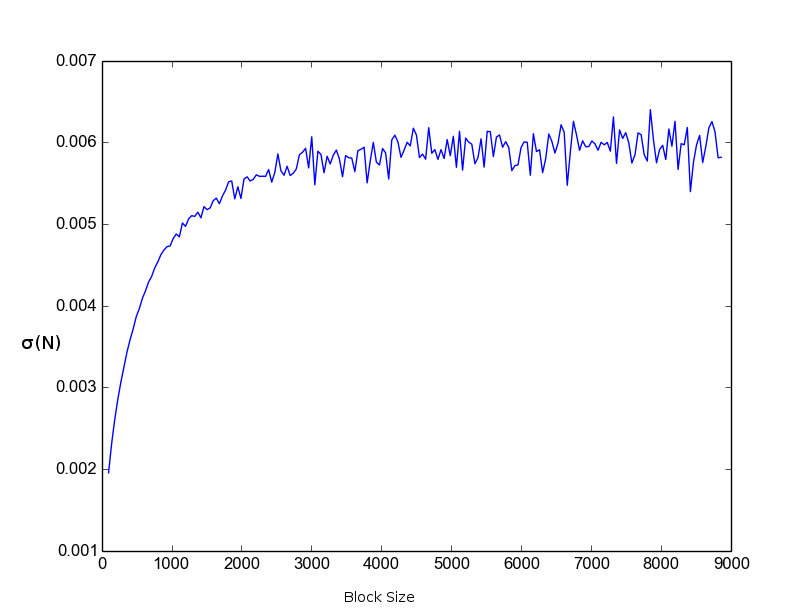
\includegraphics[width=.9\linewidth]{figure_1.png}
\caption{{\footnotesize Error as a function of the block size, the total sample was of $10^6$ points, the block size goes from 100 to 9000. The STD without blocking would be $4.5\cdot 10^-4$, while blocking adds the correlation to give a better estimate of the error, in this case $5.9 \cdot 10^-3$ which is an order of magnitude more.}}
\label{fig:fig6}
\end{figure}
\end{center}

\section*{First Tests: Non Interacting Systems}
\paragraph*{Closed Form Expressions for Expectation Values}When dealing with computational problems it's always a good practice to have some simple tests to check the code against. We will first run some tests without importance sampling. In our case we can simplify our system considerably by removing the interaction between particles. This gives us a very simple closed form expression for the ground state energy and for it's variance. We have:
\[
   E_{L}({\bf R},\alpha)=E_{K} + V_{ext} = \sum_i^N \left( -2 \alpha^2 r_i^2 + D \alpha + \frac{1}{2}r_i^2 \right)
   \label{eq:locale2}
\]
The expected value of the local energy has minimum for $\alpha =  \frac{1}{2}$, which leads to 
\[
   E_{L_{MIN}}=E_{L}({\bf R},0.5)=\frac{N D}{2}
   \label{eq:locale2}
\]
A similar approach can be applied to the variance, but this would lead to the surprising result of $\sigma ^2_{MIN} ({\bf R},0.5) = 0$, meaning that the value at $\alpha = 0.5$ is the real minimum for this Hamiltonian. These calculation consist in a very good test for our code. By trying to estimate the energy of the ground state for values around $\alpha =  \frac{1}{2}$ we can test whether the code is working correctly, especially the Metropolis algorithm part. \\
A second test is then to compute the local energy at each Monte Carlo cycle with a numeric approach, computing the double derivative numerically using the well known relation:
\[
f''(x) \approx \frac{f(x-h)-2f(x)+f(x+h)}{h^2}
\]
this method however is extremely inefficient since we have to compute derivatives in $N\cdot D$ dimension (N is the particle number and D is the number of spatial dimensions) but it's a good test in lower dimensions for comparing the data.

\noindent We first make a series of tests by varying the variational parameter and look if the minimum is at $\alpha=0.5$ as predicted by the theory.
\begin{center}
\begin{figure}[H]
 \centering
\begin{subfigure}{.5\textwidth}
  \centering
  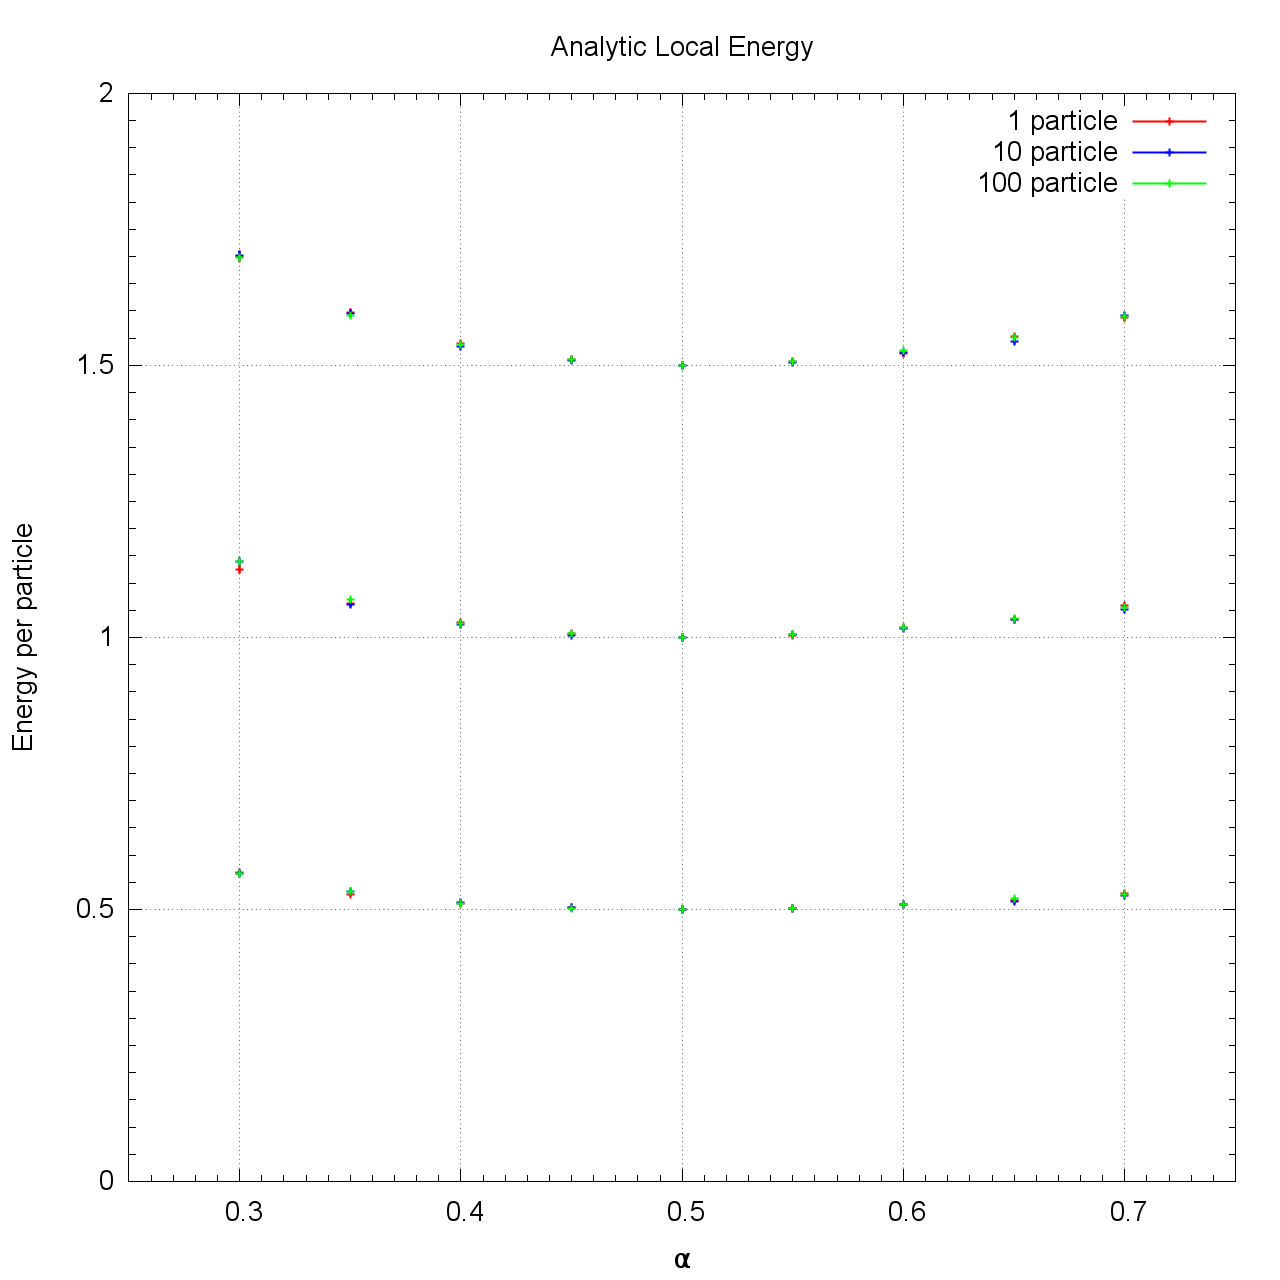
\includegraphics[width=.9\linewidth]{plot_energy.png}
  \caption{Data for 1, 10 and 100 particles computed using the \\closed form expression for the local energy.}
  \label{fig:sfig2}
\end{subfigure}%
\begin{subfigure}{.5\textwidth}
  \centering
  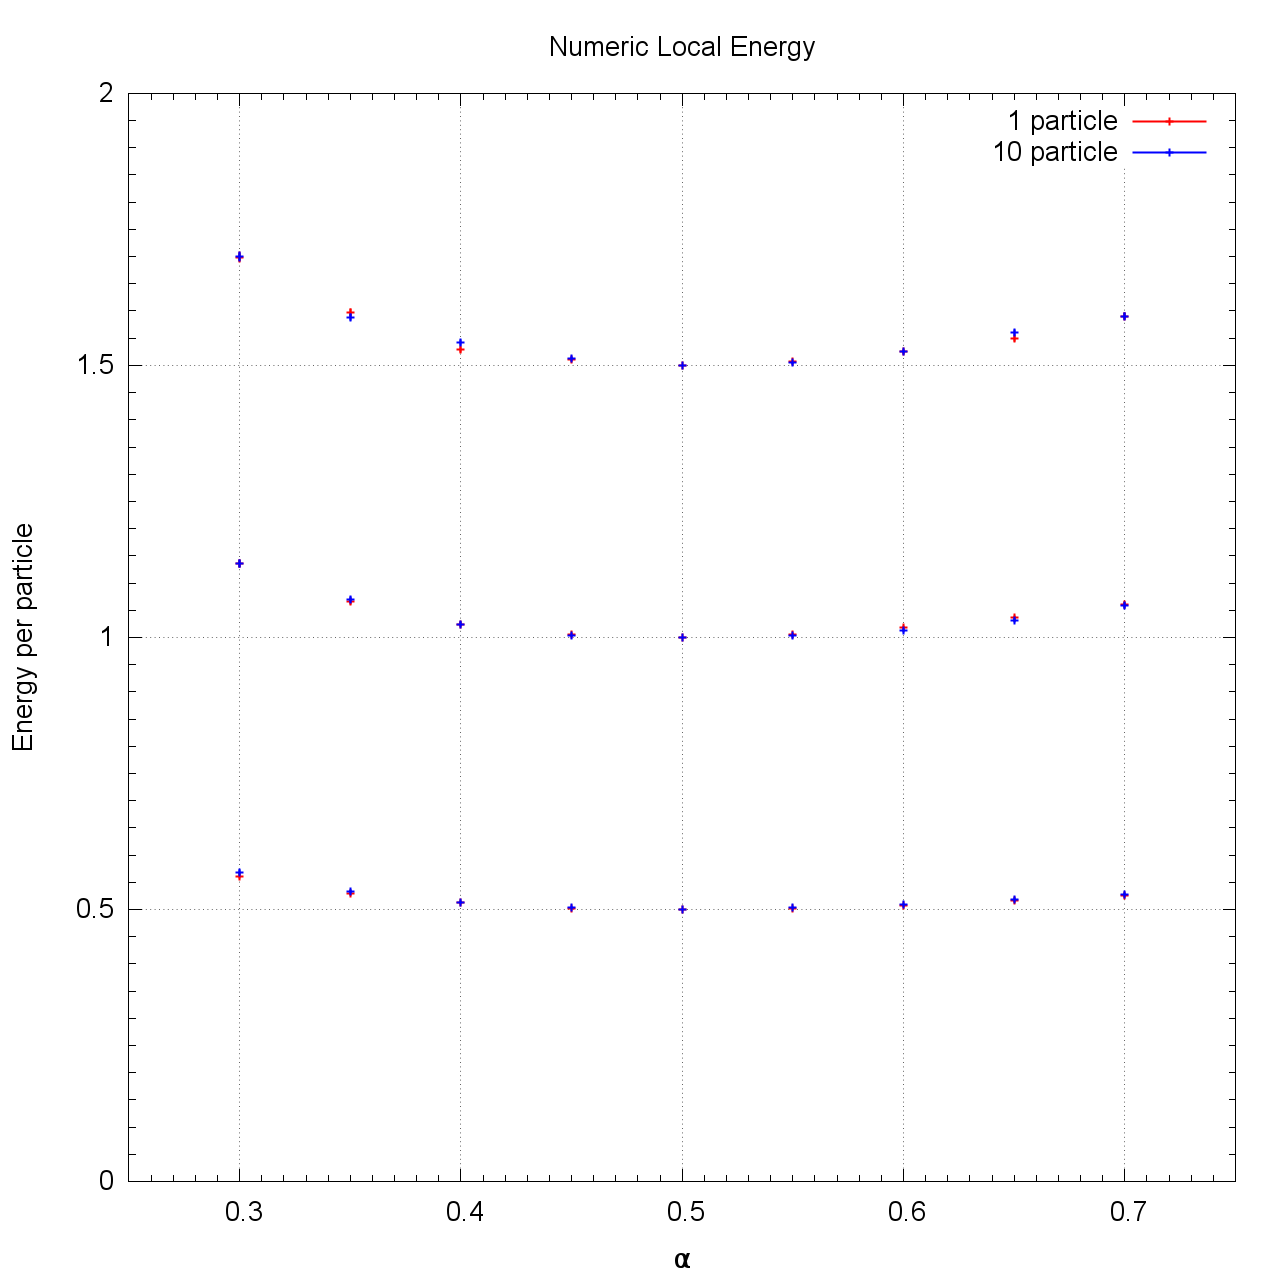
\includegraphics[width=.9\linewidth]{plot_energy_num.png}
  \caption{\footnotesize Data for 1 and 10 particles computed using numeric derivatives in the local energy.}
  \label{fig:sfig2}
\end{subfigure}%

\caption{{\footnotesize Energy of the ground state divided by the number of particles for different values of $\alpha$ around the minimum. The three different sets are for different numbers of dimensions and the relative minima are 0.5, 1, and 1.5 for 1,2,3 dimension respectively. }}
\label{fig:fig}
\end{figure}
\end{center}

Both plots show minima for $\alpha = 0.5$ for all data series. In the following table we show the data collected for 1 particle in 1 dimension for both methods and their respective variance. It's a brute force Monte Carlo calculation, with $10^6$ metropolis steps and step length $r=0.1$.\\

\begin{minipage}[b]{0.5\textwidth}\centering
\begin{table}[H]
\caption{{\footnotesize Energy and STD with closed form expressions }}
\begin{center}

\begin{tabular}[t]{c c c}
\hline
$\alpha$ & E($\alpha$) & $\sigma $(E) \\\hline 
0.30& 0.570 & 0.012 \\
0.35& 0.5339& 0.0082 \\
0.40& 0.5026& 0.0043 \\
0.45& 0.5040& 0.0022 \\
0.50& 0.5   & 0.0 \\
0.55& 0.5032& 0.0020\\ 
0.60& 0.5105& 0.0036 \\
0.65& 0.5204& 0.0054 \\
0.70& 0.5225& 0.0065 \\
\hline
\end{tabular}
\end{center}
\end{table}
\end{minipage}
\begin{minipage}[b]{0.5\linewidth}\centering
\begin{table}[H]
\caption{{\footnotesize Energy and STD with numerical derivatives }}
\begin{center}
\begin{tabular}[t]{c c c}
\hline
$\alpha$ & E($\alpha$) & $\sigma $(E) \\\hline
0.30& 0.548& 0.012 \\
0.35& 0.5195& 0.0081 \\
0.40& 0.5064& 0.0044 \\
0.45& 0.4994& 0.0023 \\
0.50& 0.5000& 3e-07 \\
0.55& 0.5027& 0.0020 \\
0.60& 0.5120& 0.0033 \\
0.65& 0.5174& 0.0052 \\
0.70& 0.5274& 0.0064 \\
\hline
\end{tabular}
\end{center}
\end{table}
\end{minipage}
With both methods the energy and the error have a minimum in 0.5, as expected, and we can see that while the numeric derivatives get really close to the values we expect, the analytic expression gets the value exactly and also the variance is 0 for the analytic form, while it doesn't vanish (though it drops to $10^-7$) for the numerical method.\\
The two methods however are definitely not equivalent. In terms of computation time having a closed form expression decreases the time by a factor of $\approx 10$ (this is a really rough estimate), which is a noticeable difference, as we increase the dimensions and the number of particles this gap gets bigger and bigger. \\
In order to make calculations using brute force Monte Carlo methods with an acceptance ratio at around 0.5, we had to use an empirical method of trial and errors in order to find the rough step size for the Metropolis cycle, which has been found around $r=4$. The whole system appeared to be very sensible to this parameter and changing this led to some inconsistent values for the energy. This implies that better sampling algorithms are needed, one of which is the importance sampling via the Metropolis-Hastings algorithm.
\paragraph*{Importance Sampling Implementation} In order to solve the previous problems we now implement the importance sampling, as discussed in the theoretical introduction. We compare the stability and acceptance ratio $A_R$ as a function of the time step $\Delta t$ with a variational parameter $\alpha$ close to the minimum value, i.e. $\alpha=0.6$, with $10^6$ Metropolis steps in the case with one particle and one dimension. The previous calculation gave in the analytic case $E(0.6)= 0.5105 \pm 0.0036$
\begin{table}[H]
\caption{{\footnotesize Importance Sampling Analysis  }}
\begin{center}
\begin{tabular}[t]{c c c c}
\hline
$\Delta t$ & $A_R$ & E(0.6) &$\sigma $(E) \\\hline
10 &0.0449 &0.5322& 0.0025 \\
1 &0.7234 &0.50855 &0.00018 \\
0.1& 0.9906 &0.50811 &0.00038 \\
0.01 &0.9997 &0.5080 &0.0012 \\
0.001 &0.9999 &0.5109 &0.0032 \\
0.0001 &1& 0.5087 &0.0059 \\
\hline
\end{tabular}
\end{center}
\end{table}
\noindent The first important result is the stability of the algorithm as a function of the  time step $\Delta t$ since the results are consistent for a wide range of the parameter.
The results indicate that the most suitable value are for $\Delta t = [0.1,1]$, for lower values the trial steps are highly correlated and the covariance (which is taken into account via the blocking technique) is high while before this value the acceptance ratio is very low. Moreover at this values the acceptance ratio is higher then the brute force Monte Carlo one but the variance is lower. Let's compare now the two algorithms with 10 particles in a 3-dimensional trap.\\

\begin{minipage}[b]{0.5\textwidth}\centering
\begin{table}[H]
\caption{{\footnotesize Importance sampling }}
\begin{center}

\begin{tabular}[t]{c c c}
\hline
$\alpha$ & E($\alpha$) & $\sigma $(E) \\\hline 
0.40&15.3794& 0.0064\\ 
0.45& 15.0812& 0.0047 \\
0.50& 15.0& 0.0\\ 
0.55& 15.0699& 0.0087\\ 
0.60& 15.729& 0.045 \\
\hline
\end{tabular}
\end{center}
\end{table}
\end{minipage}
\begin{minipage}[b]{0.5\linewidth}\centering
\begin{table}[H]
\caption{{\footnotesize Brute Force }}
\begin{center}
\begin{tabular}[t]{c c c}
\hline
$\alpha$ & E($\alpha$) & $\sigma $(E) \\\hline
0.40 &15.314 &0.021\\ 
0.45 &15.0824 &0.0099 \\
0.50 &15.0 &0.0\\ 
0.55 &15.0691 &0.0079\\ 
0.60 &15.230 &0.016 \\
\hline
\end{tabular}
\end{center}
\end{table}
\end{minipage}
Comparing the two data sets we are not able to find evident differences between the results given with the two different metropolis Algorithm and even if we repeat the same experiment we get the values:

\begin{minipage}[b]{0.5\textwidth}\centering
\begin{table}[H]
\caption{{\footnotesize Importance sampling }}
\begin{center}

\begin{tabular}[t]{c c c}
\hline
$\alpha$ & E($\alpha$) & $\sigma $(E) \\\hline 
0.40&15.3666& 0.0066\\ 
0.45& 15.0845& 0.0046 \\
0.50& 15.0& 0.0\\ 
0.55& 15.070& 0.008\\ 
0.60& 15.980& 0.052 \\
\hline
\end{tabular}
\end{center}
\end{table}
\end{minipage}
\begin{minipage}[b]{0.5\linewidth}\centering
\begin{table}[H]
\caption{{\footnotesize Brute Force }}
\begin{center}
\begin{tabular}[t]{c c c}
\hline
$\alpha$ & E($\alpha$) & $\sigma $(E) \\\hline
0.40& 15.370 &0.021\\ 
0.45& 15.0742 &0.0091\\
0.50& 15.0 &0.0 \\
0.55& 15.0618& 0.0079\\ 
0.60& 15.241& 0.015 \\
\hline
\end{tabular}
\end{center}
\end{table}
\end{minipage}
By a fast check we can see that at these fixed step parameters both algorithms look stable, moreover the two sets of data are compatible within their framework using the computed variance, this is an effective test that we can trust the values of the variance that we are computing. An experiment with more Monte Carlo Cycles is needed in order to have a better comparison of these two algorithms.\\
Even though we haven't found any effective change in the data between the two algorithms we can assert that Importance Sampling is a better choice since gives stable results for a wider range of the step parameter.  

\section*{Elliptic Trap}
\noindent We now unify all the previous steps in order the make a complete variational Monte Carlo Calculation of an interacting boson gas trapped in a elliptic potential trap. In order to benchmark our calculation we'll set the system having an interaction length $a=0.0043$ and the harmonic potential along z being $\gamma^2$ stronger(with $\gamma=2.82843$) then the other directions. Then the Hamiltonian of the system can be rewritten as: 
 \begin{equation}
H=\sum_{i=1}^N\frac{1}{2}\left(-\nabla^2_i+x_i^2+y_i^2+\gamma^2 z_i^2\right)+\sum_{i<j}V_{int}(|{\bf r}_i-{\bf r}_j|).
\end{equation} 
we make our calculation with $N=10,50,100$ particles and compare it with the literature. By repeating the calculations done in the previous sections we get a correction for the energy expectation value:
\[
   E_{L}({\bf R},\alpha)=E_{K} + V_{ext} = \sum_i^N \left( -2 \alpha^2 (x_i^2+ y_i^2 + \beta ^2 z_i^2) + D \alpha + \frac{1}{2}(x_i^2+ y_i^2 + \gamma ^2 z_i^2) \right)
   \label{eq:locale2}
\]
by setting $\beta=\gamma=2.82843$\footnote{We took this value because we had some benchmarks to compare our results with.} the minimum for the local energy should still be found for $\alpha = 0.5$. We ran a calculation using $10^6$ Monte Carlo cycles, without interaction for $N=10,50,100$ and plotted the results:
\begin{center}
\begin{figure}[H]
 \centering
  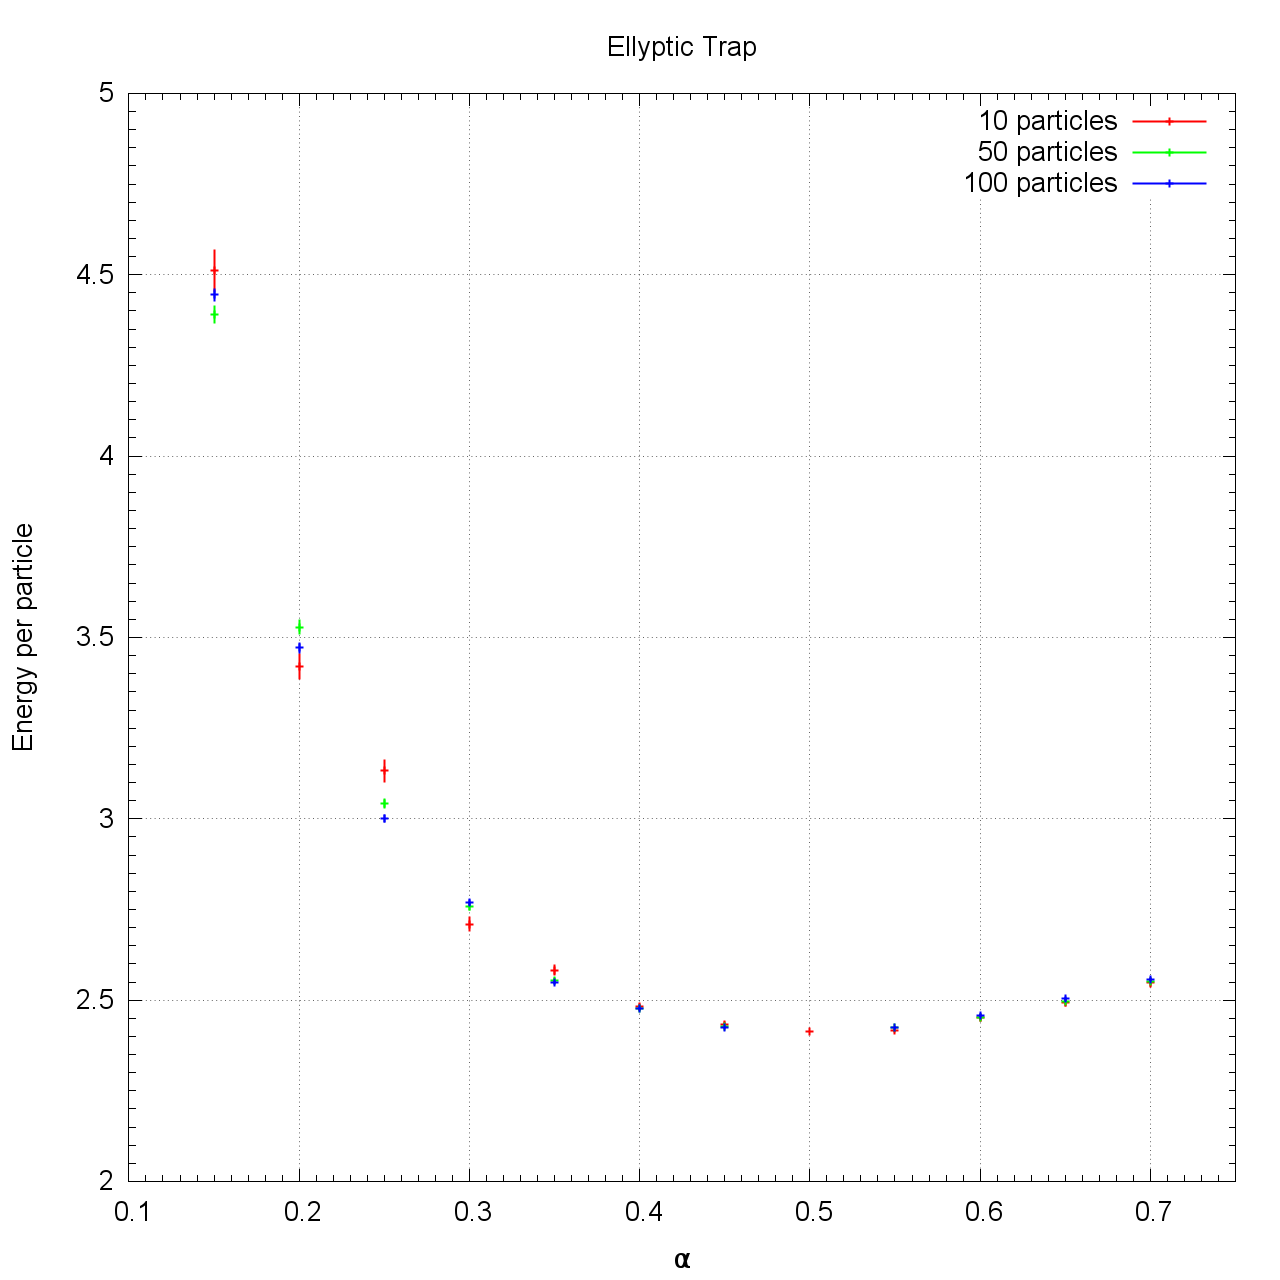
\includegraphics[width=.9\linewidth]{plot_ellyptic.png}
\caption{{\footnotesize Energy of the ground state per particle as a function of $\alpha$ for a elliptic harmonic oscillator ($\omega z = \gamma \omega_{x,z}$ and a trial wave function $\Psi_{T}( {\bf{R}, \alpha, \beta}$) with $\beta = \gamma = 2.82843$. Ran with $10^6$ Monte Carlo cycles for systems of 10, 50 and 100 particles.}}
\label{fig:fig6}
\end{figure}
\end{center}
The plot shows a similar curve as for the spherical trap, but with higer energy per particle than before. This is due to the fact that the same mean position in the two oscillators give very different energies, as the elliptical trap is basically enlarging the potential in one direction by a factor of $\approx 8$.\\
In literature (Ref . 2) we found some data regarding this same problem. We used these data as a benchmark for the goodness of our code. 
\begin{table}[H]
\caption{{\footnotesize Data Comparison between benchmark on Ref[1] and our data }}
\begin{center}
\begin{tabular}[t]{c c c c c c c }
\hline
Number of Particles & \multicolumn{2}{c}{N = 10 }  & \multicolumn{2}{c}{N = 50 }     &  \multicolumn{2}{c}{N = 100 }  \\\hline
alpha &  Benchmark  &  Computed  &  Benchmark  &  Computed  &  Benchmark  &  Computed  \\\hline
0.2   & 34.9   & 34.88 $\pm$ 0.34 & 175   & 176.38 $\pm$ 0.87 &       353 & 347.18 $\pm$ 1.24 \\
0.3   & 24.7   & 27.50 $\pm$ 0.18 & 138   & 137.94 $\pm$ 0.38 &      278 & 276.99 $\pm$ 0.53 \\
0.4   & 24.2   & 24.69 $\pm$ 0.07 & 125   & 123.88 $\pm$ 0.17 &      253 & 247.67 $\pm$ 0.26 \\
0.5   & 24.2   & 24.14 $\pm$ 1.51 $\cdot$ 10$^-7$ & 122   & 120.71 $\pm$ 0 &      247 & 241.42 $\pm$ 0    \\
0.6   & 24.6   & 24.59 $\pm$ 0.05 & 125   & 122.62 $\pm$ 0.13 &      252 & 242.40 $\pm$ 0.10 \\
0.7   & 25.5   & 25.46 $\pm$ 0.09 & 129   & 127.62 $\pm$ 0.23 &      263 & 255.73 $\pm$ 0.31 \\\hline

\end{tabular}
\end{center}
\end{table}
\noindent The two data sets appear to be very similar and this means that our programs is working correctly, at least for the non interacting part. The differences in the data points could be given by the number of Monte Carlo cycles used for each point, ours was quite low (just $10^6$ for $N=10,50$ and $10^5$ for $N=100$). Another cause of discrepancy could be the steplength parameter, which, to some extent, on low number of cycles can influence the outcome of the calculations. \\
Nevertheless, the behavior of the system seems to be fairly equal, having the minimum in $\alpha = 0.5$ with no dependency on the number of particles. Since we are also neglecting the interactions, the energy per particle is also independent from the size of the system as expected.\\

\section*{Interaction: Jastrow Factor}
\noindent One of the main points of the calculation was to implement the interaction between the bosons. This comes in with the Jastrow factor in the wave function and it's the most demanding term both to program and to compute. Without the interaction the execution time scales as $N$ more or less, since there are no loops over the pair of particles. With the interaction it scales as $N^2$, since in the second derivative of the wave function (needed for the local energy) the interaction term leads to a double loop in the number of particles.
Physically we are expecting higher ground state energies than before, since now the particles can't stack up in the middle of the harmonic oscillator trap because of the repulsion they are subjected to. We also expect the energy to move further apart from the ideal case for larger number of particles. \\
One last difference between the interacting and non-interacting case is that the minimum of the energy is not necessarily given by $\alpha = 0.5$. This value won't change much, but the difference should be noticable.\\
In order to quantify the influence of the interaction, we decided to plot the ratio between the energy computed with interaction over the non-interacting one. We calculated this quantity for both the spherical and the elliptical trap. \\
In the following plot we show the previously described ratio for both systems shapes:
\begin{center}
\begin{figure}[H]
 \centering
\begin{subfigure}{.5\textwidth}
  \centering
  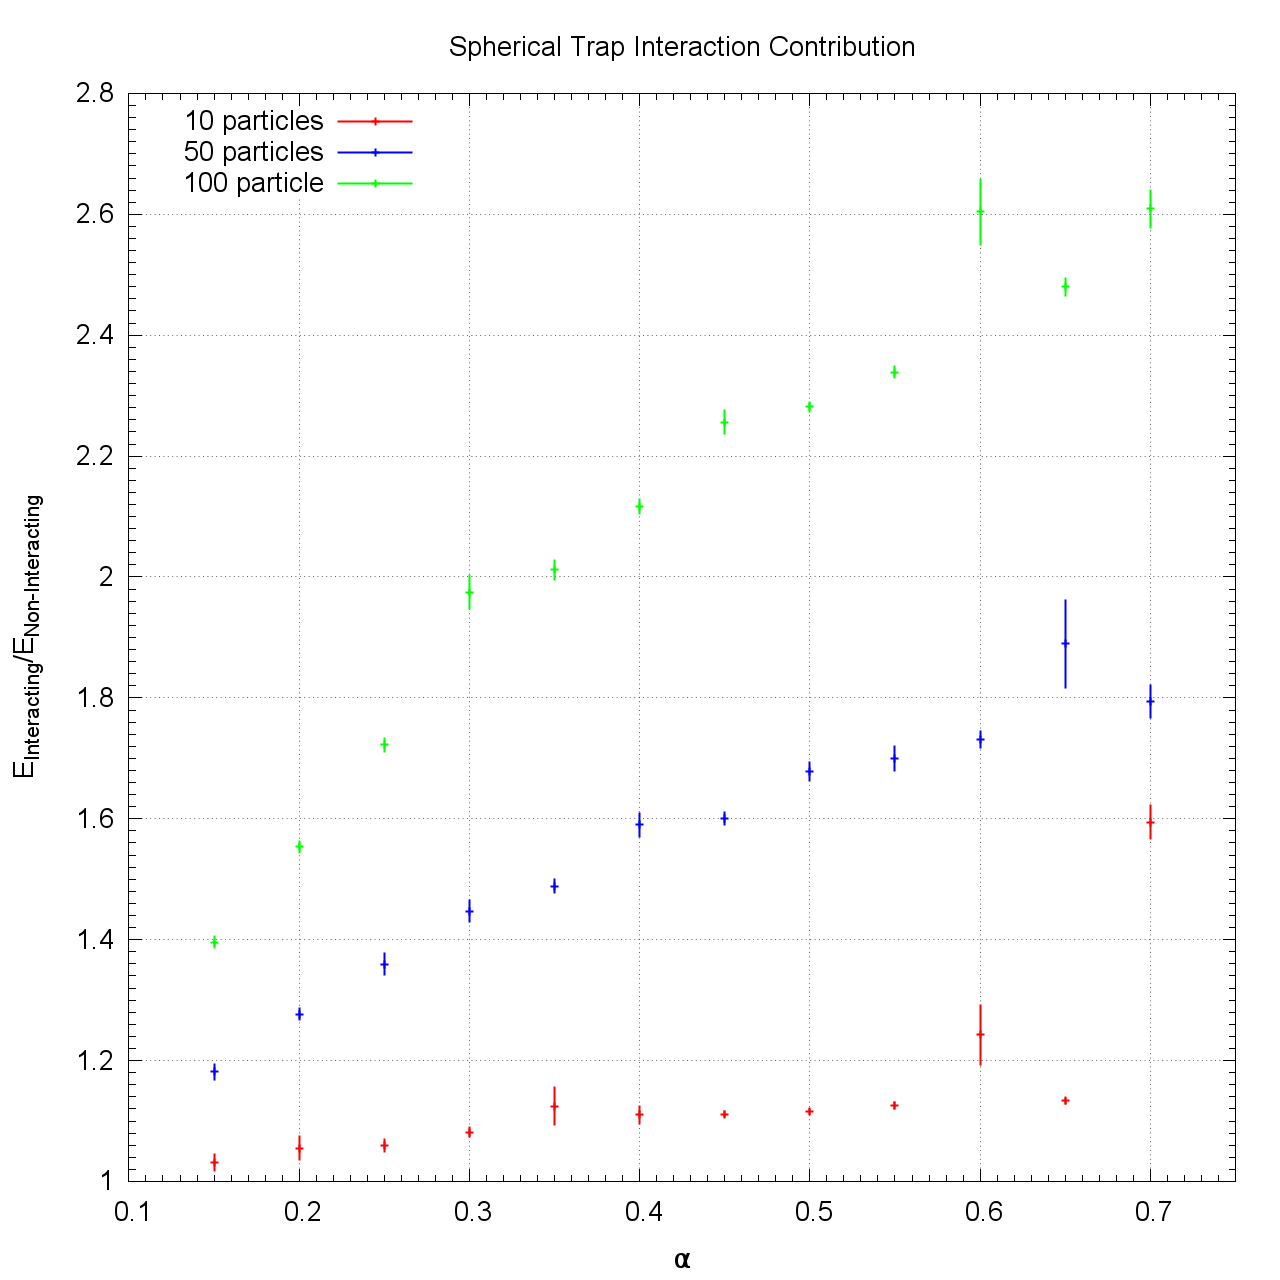
\includegraphics[width=.9\linewidth]{plot_jastrow_sphere.png}
  \caption{\footnotesize Data for 10, 50 and 100 particles computed using the \\spherical harmonic oscillator potential, with and without the \\Jastrow factor and taking the ratio.}
  \label{fig:sfisfdg2}
\end{subfigure}%
\begin{subfigure}{.5\textwidth}
  \centering
  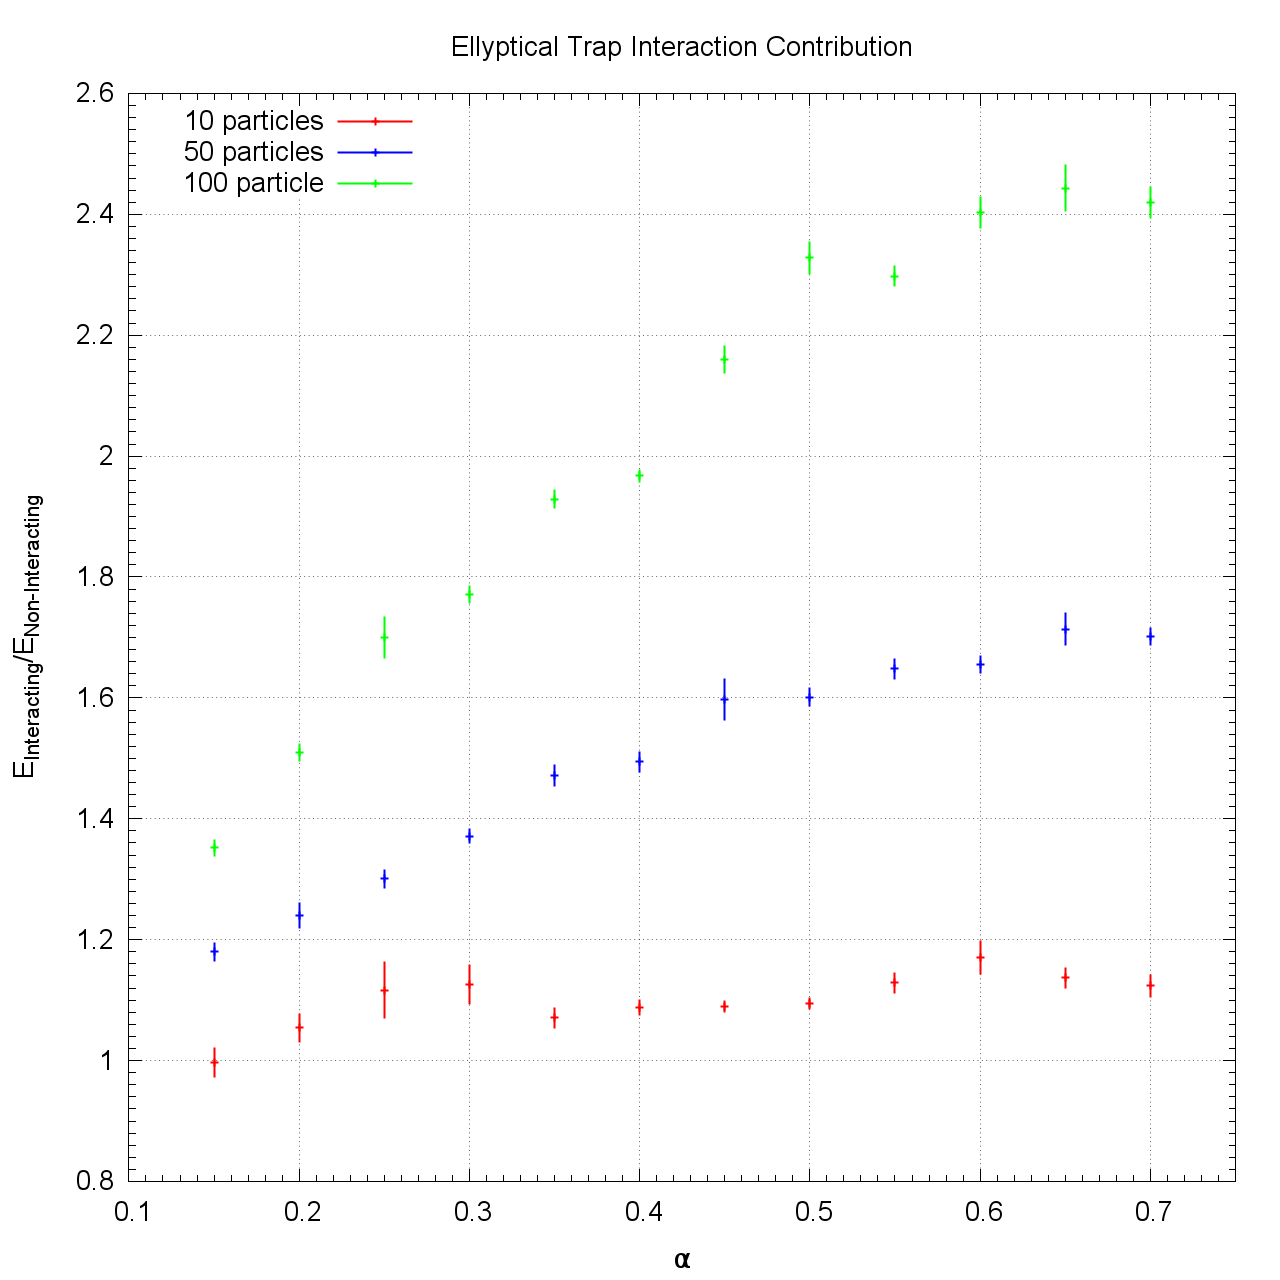
\includegraphics[width=.9\linewidth]{plot_jastrow_ellipse.png}
  \caption{\footnotesize Data for 10, 50 and 100 particles computed using the elliptic harmonic oscillator potential, with and without the Jastrow factor and taking the ratio.}
  \label{fig:sfifdsg2}
\end{subfigure}%
\end{figure}
\end{center}
We immediately see that by increasing the number of particles the correlation term becomes more and more important, leading to energies that are on average double for 100 particles,but almost the same for just 10. The alpha dependency of the ratio can be explained by the fact that for larger $\alpha$ we have smaller average distance between the particles, and viceversa, so for smaller values of the variational parameter the interaction is less relevant than for higher values. This implies that also the minimum of the energy is moved to a smaller value of $\alpha$ than before, but this will be discussed in the next section.

\section*{Interaction: Conjugate gradient}
\noindent Since now we have taken into account the interaction between the particles the optimal variational parameter $\alpha$ must be slightly changed from the previous value at $\alpha_{min}=0.5$. For finding the new optimal parameter we have been trying to use the conjugate gradient algorithm but the we haven't been able to find any stable and distinct value within the uncertainty, however by looking at the wave function we expect the variational parameter to be slightly smaller since the average distance will be incremented by the repulsion between the particles.
However with the given value of the interaction length $a=0.0043$ we have been performing a rough study of the variational parameter knowing that the value must be close to the minimum.
% * <giulioisac@gmail.com> 2016-03-21T09:49:06.932Z:
%
% > However with the given value of the interaction length $a=0.0043$ we have been performing a rough study of the variational parameter knowing that the value must be close to the minimum.
%
% ^.
\section*{Conclusions}
\noindent Our work managed to reproduce results for a similar problem within a very small discrepancy interval. Moreover the results that couldn't be checked in literature follow the physical behavior of the system and this allows us to suppose that our code is working properly. \\
Blocking was proven to be absolutely necessary, since it gives a real estimate of the error and not just the STD. In many cases the difference was 1 or 2 orders of magnitude.\\
The conjugate gradient method however didn't give us the results we would have expected, perhaps this is just a matter of sensibility to the initial parameters or the low MC cycles we were using.\\
Due to the very high level of modularity given by object-oriented C++, our code can now be used to simulate many different systems with very few corrections, we could example by introducing anti-symmetrical conditions, switch to a gas of fermions. Other developments would be adding parallelization, which should be straightforward, to allow the code to run on clusters to be able to increase enormously the number of Monte Carlo cycles. 

\section*{References}
\begin{enumerate}
\item J.~L.~DuBois and H.~R.~Glyde, H. R., {\em Bose-Einstein condensation in trapped bosons: A variational Monte Carlo analysis},
Phys.~Rev.~A {\bf 63}, 023602 (2001).

\item J.~K.~Nilsen,  J.~Mur-Petit, M.~Guilleumas, M.~Hjorth-Jensen, and A.~Polls, {\em Vortices in atomic Bose-Einstein condensates in the large-gas-parameter region},
Phys.~Rev.~A {\bf 71}, 053610 (2005).

\item Github address : \url {https://github.com/GioPede/FYS4411/tree/master/Project1}

\end{enumerate}
\end{document}